\documentclass[11pt,a4paper]{article}
\usepackage[utf8]{inputenc}
\usepackage[T1]{fontenc}
\usepackage{lmodern}
\usepackage[margin=2.5cm]{geometry}
\usepackage{amsmath,amssymb}
\usepackage{booktabs}
\usepackage{graphicx}
\usepackage{xcolor}
\usepackage{url}
\usepackage[colorlinks=true,linkcolor=blue!50!black,citecolor=blue!50!black,urlcolor=blue!50!black]{hyperref}

\newcommand{\R}{\mathbb{R}}

\title{Ill-conditioning of the discrete inverse conductance problem as exponential dependence on the earlier span:\\ a column-residual certificate, partly machine-checked, and its measurement}
\author{Xavier Callens\\[2pt]
\small SocrateAI Lab, Cagnes-sur-Mer, France\\
\small \texttt{callensxavier@gmail.com}}
\date{October 2026 \\ \small Preprint, not peer reviewed. Companions: doi:10.5281/zenodo.23228685, doi:10.5281/zenodo.23241463, doi:10.5281/zenodo.23244556}

\begin{document}
\maketitle

\begin{abstract}
The companion preprints measured the exponential growth of the condition number of the Jacobian of the Dirichlet-to-Neumann map of a resistor network with respect to its edge conductances, with the depth of the unknowns, and found
that persistent homology of the nearest-neighbour structure of the Jacobian columns sees the depth only through a slow power law. Here we measure the quantity that carries the rate: the distance of a column to the span of the columns that precede it when
the columns are ordered by depth. Two elementary facts bound the smallest singular value above by such residuals; one of them is machine-checked in Lean 4 (a lower bound on the action of the matrix is at most every column residual), the other is the standard leave-one-out identity.
On a square disk the minimum depth-ordered residual of each layer falls $1.243$ decades per layer against $1.272$ for the smallest singular value (ratio $0.977$, preregistered band $0.85$ to $1.15$), and the median column, not only the worst, falls exponentially ($0.656$ decades per layer, correlation $-0.999$),
seven times faster than the nearest-neighbour topology. Dependence within the layer itself costs a further $0.6$ to $1.8$ decades at each layer, more than a pilot suggested (a preregistered bound was refuted). On the $\{7,3\}$ tiling the worst column falls $0.40$ decades per layer over four layers, a third of the square's rate, and most columns remain well separated.
Two design errors of mine (an explicit Jacobian too large for memory, bands set from a smaller pilot) are kept in the record. Nothing here concerns holography or noise.
\end{abstract}

\section{Introduction}
The condition number of the Jacobian $J$ of the Dirichlet-to-Neumann (DtN) map of a resistor network, one column per edge conductance, grows exponentially with the depth of the edges on flat lattice disks and slowly on hyperbolic tilings~\cite{Preprint};
exponential ill-conditioning of the inverse conductivity problem is classical~\cite{DiCristoRondi,BorceaReview}. The first companion gave an exact rate on a solvable strip~\cite{StripPaper}. The second asked what persistent homology sees in the cloud of Jacobian columns and found that the median $H_0$ death time of a depth layer, the typical angle between
neighbouring columns, falls only like one over the depth while $\sigma_{\min}$ falls exponentially~\cite{Paper2}; its reading was that the dependence responsible for the small singular value is spread over many columns and invisible to nearest neighbours. This note tests that reading with the quantity that measures such dependence directly and that bounds $\sigma_{\min}$.

\section{Exact facts}\label{sec:exact}
Let $J$ have columns $a_1,\dots,a_n$, sorted by depth, and let $\sigma$ satisfy $\sigma\|x\|\le\|Jx\|$ for all $x$ (so $\sigma\le\sigma_{\min}$ if $J$ has full column rank).
\begin{enumerate}
\item \emph{Column-residual bound.} For every $j$ and every coefficient vector $y$ with $y_j=0$, $\sigma\le\|a_j-\sum_iy_ia_i\|$. Proof: apply the hypothesis to $x=e_j-y$, whose norm is at least $1$. This is formalised in Lean 4 against Mathlib (\texttt{le\_residual}); the identification of such a $\sigma$ with $\sigma_{\min}$ and the passage to the distance to the span are not formalised.
\item \emph{Leave-one-out identity.} The distance $r_j$ of $a_j$ to the span of the other columns satisfies $r_j^2=1/(G^{-1})_{jj}$ with $G=J^{\top}J$; hence $\sigma_{\min}\le\min_jr_j$ and $\min_jr_j/\sqrt n\le\sigma_{\min}$. This is standard linear algebra; no citation is claimed and it is not formalised.
\item \emph{Nested spans.} The depth-ordered residual $\rho_j=|R_{jj}|$ of the QR factorisation of the depth-sorted matrix (the distance to the span of the preceding columns) satisfies $\rho_j\ge r_j$, and the distance $s_e$ to the span of the strictly shallower layers satisfies $s_e\ge\rho_e$.
\end{enumerate}
So $\sigma_{\min}(J_{\le k})\le\min_jr_j\le\min_{j\in\text{layer }k}\rho_j\le\min_{e\in\text{layer }k}s_e$, a chain checked numerically (gate G1). Three further elementary lemmas are machine-checked in the same Lean project: the DtN matrix of a symmetric matrix with zero row sums and invertible interior block is symmetric and has zero row and column sums,
and row and column offsets are Frobenius-orthogonal to matrices with zero sums. Gates (build, search for \texttt{sorry}, axiom audit with only the three standard axioms, statement lock) passed, and a separate agent audited the wording of the docstrings; the audit led to corrections of overstatements, listed in the repository.

\section{Measurement}\label{sec:measure}
The columns are $J_e=\mathrm{upper}(d_ed_e^{\top})$ as in the companions. For the square disk of radius 16 we compute Householder QR of the explicit Jacobian with columns sorted by depth, and, per layer, $\sigma_{\min}(J_{\le k})$ by singular value decomposition, the leave-one-out minimum from $R^{-1}$, the minimum $\rho$, the minimum $s$, and the median of $s_e/\|J_e\|$.
The scored layers are those $k\ge2$ with $\sigma_{\min}\ge10^{-12}$ (layers $2$ to $7$). For the $\{7,3\}$ tiling with five layers the explicit Jacobian does not fit in memory (my design error, below), so the same quantities are computed from the column Gram matrix by Cholesky factorisation, valid because the condition number there is about $10^4$; the two routes agree to $2\times10^{-8}$ on a test disk.
Preregistration 32 (committed before the run, with a disclosed pilot at radius 10 that informed the bands) fixed six predictions.

\paragraph{Results} (Table~\ref{tab:layers}, Figure~\ref{fig:res}, Table~\ref{tab:register3}). The exact chain held on every layer. The depth-ordered minimum carries the rate: slope $-1.243$ against $-1.272$ for $\sigma_{\min}$, and the leave-one-out minimum $-1.263$; the gap between $\rho$ and $\sigma_{\min}$ is $0.61$ to $1.39$ decades.
The median relative distance to the shallower span falls $0.656$ decades per layer (correlation $-0.999$), seven times the slope of the nearest-neighbour $H_0$ death times of the previous note. The prediction that the gap between the distance to the shallower span and $\rho$ stays below $1.5$ decades was \emph{refuted}: it reaches $1.81$ at layer 5 (mean $1.23$; the pilot had shown at most $1.2$).
On the $\{7,3\}$ tiling the minimum $\rho$ falls $0.40$ decades per layer over layers $1$ to $4$ (slope of $\sigma_{\min}$: $0.39$), the gaps are small ($0.09$ to $0.37$), and the median relative residual is $0.89$, $0.54$, $0.55$, $0.35$.

% GENERATED by make_paper3.py from data/*.json -- do not edit
\begin{table}[t]\centering\small
\caption{Square disk (radius 16), scored layers: $\sigma_{\min}$ of $J_{\leq k}$, minimum leave-one-out residual (LOO), minimum depth-ordered residual $\rho$, minimum distance $s$ to the span of strictly shallower layers, and the median of $s/\|J_e\|$ over the layer. Below the rule: the $\{7,3\}$ tiling with five layers (Gram route).}
\label{tab:layers}
\resizebox{\linewidth}{!}{%
\begin{tabular}{ccccccc}\toprule
Layer & edges & $\log_{10}\sigma_{\min}$ & $\log_{10}$ LOO & $\log_{10}\rho$ & $\log_{10}s$ & median $s/\|J_e\|$ \\ \midrule
2 & 148 & -4.842 & -4.386 & -3.855 & -3.236 & 0.174 \\
3 & 140 & -6.179 & -5.760 & -5.127 & -4.202 & 0.051 \\
4 & 132 & -7.406 & -6.959 & -6.597 & -5.305 & 0.011 \\
5 & 124 & -9.260 & -8.788 & -8.651 & -6.840 & 0.002 \\
6 & 108 & -10.154 & -9.671 & -8.760 & -7.349 & 0.000 \\
7 & 100 & -10.991 & -10.515 & -9.964 & -8.632 & 0.000 \\
\midrule
1 & 532 & -2.115 & -1.906 & -1.804 & -1.375 & 0.887 \\
2 & 147 & -2.279 & -2.186 & -2.186 & -2.156 & 0.538 \\
3 & 203 & -3.101 & -2.822 & -2.727 & -2.437 & 0.549 \\
4 & 56 & -3.145 & -2.962 & -2.960 & -2.945 & 0.350 \\
\bottomrule\end{tabular}}\end{table}

\begin{table}[t]\centering\small
\caption{Gates and predictions of preregistration 32, from the stored verdicts. Slopes in decades per layer: sigma min -1.272, rho -1.243, loo min -1.263, s min -1.084, median rel s -0.656.}
\label{tab:register3}
\begin{tabular}{lll}\toprule
Item & Verdict & Value \\ \midrule
G1 exact chain & pass &  \\
G2 QR reconstruction & pass & 3.4e-16 \\
G3 leave-one-out identity & pass & 1.6e-14 \\
G4 Gram route (added) & pass & 2.0e-08 \\
P1 rate captured & held & ratio 0.977 \\
P2 looseness of $\rho$ & held & gaps 0.61 to 1.39 \\
P3 same layer versus depth & refuted & gaps 0.62 to 1.81, mean 1.23 \\
P4 median residual exponential & held & slope -0.656, Pearson -0.999 \\
P5 hyperbolic & held & slope -0.401 against -1.243 \\
P6 contrast with nearest neighbours & held & ratio 7.3 \\
\bottomrule\end{tabular}\end{table}


\begin{figure}[t]\centering
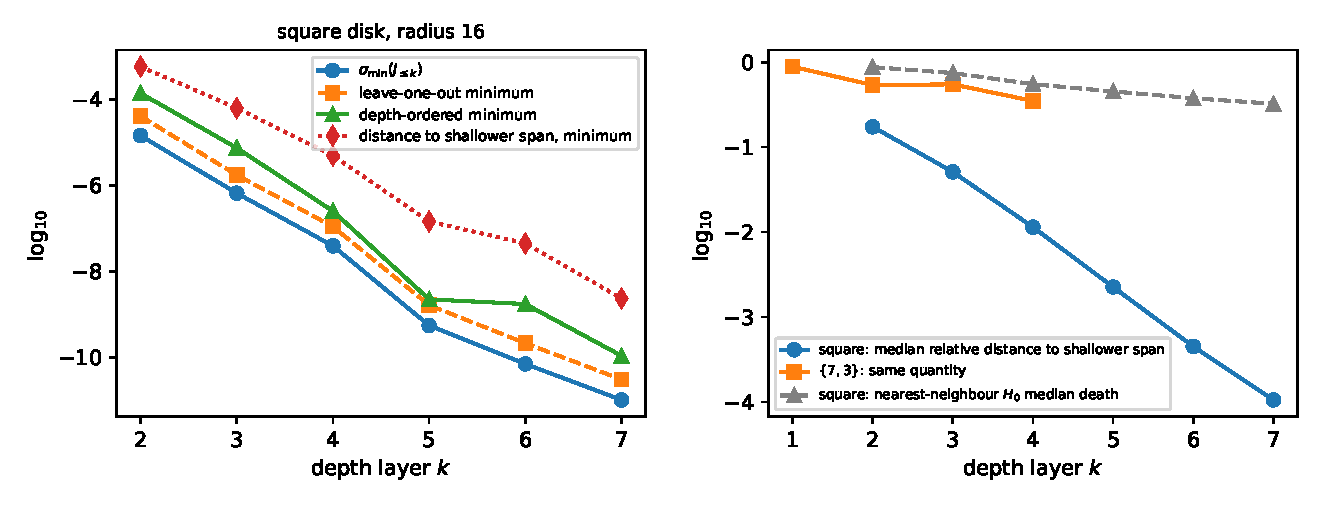
\includegraphics[width=0.98\linewidth]{fig_p3_residuals.pdf}
\caption{Left: square disk, $\log_{10}$ of $\sigma_{\min}(J_{\le k})$, the leave-one-out minimum, the depth-ordered minimum $\rho$ and the minimum distance to the shallower span, by layer. Right: median relative distance to the shallower span on the square disk and on $\{7,3\}$, and the nearest-neighbour $H_0$ median death time of the previous note.}
\label{fig:res}
\end{figure}

\paragraph{Reading.} Ill-conditioning of this problem is not a nearest-neighbour phenomenon. A deep column lies in an exponentially thin cone around the span of the shallower ones, and the cone is visible only when the whole earlier span is accounted for, as the Gram--Schmidt residual does and persistent homology of the pairwise cloud does not.
The depth-ordered residual is a cheap, certified upper bound that tracks $\sigma_{\min}$'s rate to within 3\,\% here, and it separates the contribution of depth from that of the layer itself. On the hyperbolic tiling the worst column still decays, at a third of the square's rate, while the typical column stays well separated; four layers cannot distinguish a polynomial from a slow exponential.

\section{What failed}
\begin{itemize}
\item Two launches of the experiment were killed by the operating system for memory: the preregistration asked for the explicit Jacobian on the $\{7,3\}$ tiling with five layers, which has about a million rows. I had met the same limit in the previous note and did not carry the lesson over. The hyperbolic part was moved to the Gram route by a recorded deviation before any number existed, with a new gate.
\item The bound of $1.5$ decades on the cost of same-layer dependence was informed by a pilot on a smaller disk and was too tight at radius 16.
\item The first compile of the new Lean module failed on two points (a rewrite in the wrong direction for the inverse of a transpose, and a renamed constant), repaired before any statement was locked.
\end{itemize}

\section{Limits}
Double precision, direct current, one square disk and four hyperbolic layers, no noise. The certificate bounds $\sigma_{\min}$ from above and says nothing about stability under measurement noise. The Lean statements are elementary; the identification of the Jacobian columns with the objects in them is not formalised.
The runs were recorded by the orchestrating model directly and are not entered in the evidence ledger. Nothing here concerns holography.

\section*{Reproducibility}
Script \texttt{exp32}, preregistration 32 with its deviation, the pilot scripts, the data file under \texttt{data/}, the generator \texttt{paper/make\_paper3.py} and the Lean project \texttt{lean/dtn\_offsets} are in the repository of the companion preprint. Every table and figure is generated from the stored data.

\section*{Use of AI tools}
Code, numerical experiments, the Lean files and drafting were carried out with the assistance of Claude (Anthropic); the Lean wording was audited by a separate model instance. The author directed the work and takes responsibility for the content.

\begin{thebibliography}{99}
\bibitem{Preprint} X.~Callens, Logarithmic boundary depth and the conditioning of the discrete inverse conductance problem on hyperbolic lattices (version 1.2), Zenodo, doi:10.5281/zenodo.23228685.
\bibitem{StripPaper} X.~Callens, Exact exponential rates for the discrete Calder\'on problem on lattice strips, and what transient data do not change, Zenodo, doi:10.5281/zenodo.23241463.
\bibitem{Paper2} X.~Callens, A topological proxy for the ill-conditioning of the discrete inverse conductance problem, and an independent integrator check of a resistor--capacitor bench, Zenodo, doi:10.5281/zenodo.23244556.
\bibitem{DiCristoRondi} M.~Di Cristo and L.~Rondi, Examples of exponential instability for elliptic inverse problems, arXiv:math/0303126 (2003).
\bibitem{BorceaReview} L.~Borcea, V.~Druskin, F.~Guevara Vasquez and A.~V.~Mamonov, Resistor network approaches to electrical impedance tomography, in \emph{Inside Out II}, MSRI Publications 60 (2012); arXiv:1107.0343.
\end{thebibliography}
\end{document}
